   %Dokumentinformationen	======================================================================
\newcommand{\titleinfo}{Analysis 2b - Formelsammlung}
\newcommand{\authorinfo}{Dev4Future \& S.Walker, sowie weiter Autoren}
\newcommand{\versioninfo}{$ FS \ 2019 $}
\newcommand{\licence}{CC BY-NC-SA}

%Auflistung der Autoren
%Stefan Steiner auf Vorlage von F. Braun, R.Koller, L.Leuenberger und weiteren
%An den Stoff von An2b angepasst von S. Walker und Dev4Future

%eigene Befehle: ==========================================================================
%weitere neue oder umdefinierte Befehle 
\newcommand{\fb}[1]{\textcolor{red}{\textit{#1}}}	%Verweis auf Seite im Formelbuch

% Die Verweise auf das Formelbuch beziehen sich auf den Bronstein 10. Auflage

%Tabellen Höhe
\renewcommand{\arraystretch}{2}


% standard header
%Darstellung Dokument =========================================================================================

\documentclass[10pt,twoside,a4paper,fleqn]{article}			%\documentclass[Optionen]{Dokumentklasse} => [Schriftgrösse, Layout, Papierformat, Gleichungen Linksbündig]{Art des Dokuments}
\usepackage[left=5mm,right=5mm,top=5mm,bottom=2.5mm,includeheadfoot]{geometry}	%Seitenränder festlegen


%wichtige Standard-Packages ===================================================================================

%Darstellung Text
\usepackage[utf8]{inputenc}		%LaTeX arbeitet standardmässig mit der "normalen" ASCII Codierung. Um Sonderzeichen verwenden zu können, muss deshalb explizit die UTF-8 Codierung eingestellt werden. Dazu wird das inputenc Package benötigt.
\usepackage[T1]{fontenc}		%Um die Schriftart so zu laden, dass alle Sonderzeichen nach west-europäischem Standard zur Verfügung stehen, muss die Font Encoding auf "T1" eingestellt werden:
\usepackage[ngerman]{babel}		%Das babel Paket stellt eine verbesserte Silbentrennung zur Verfügung. Wichtig ist, dass die richtige Sprache ausgewählt wird. In der Regel werden english oder ngerman (n für neue Rechtschreibung) verwendet.


%Mathematik
\usepackage{amsmath}		%Das amsmath Paket der American Mathematical Society stellt erweiterte Mathematik Zeichen, Operationen und Umgebungen zur Verfügung.
\usepackage{array}			%Definiert die array-Umgebung, die im mathematischen Modus zur Erzeugung von Matrizen dient.
\usepackage{amssymb}		%Zusätzliche Mathematische Symbole wie zum Beispiel der Implikationspfeil oder Mengen-Buchstaben, siehe auch: http://milde.users.sourceforge.net/LUCR/Math/mathpackages/amssymb-symbols.pdf

	
	
%weitere Darstellungen
\usepackage{fancybox}	%bietet mehr Möglichkeiten, wie Textboxen benutzt werden können
\usepackage{color}
\usepackage{multicol}	%Diese Umgebung erlaubt, Teile des Dokumentes mehrspaltig zu setzen.
\usepackage{verbatim}	%Macht mehrzeilige Kommentare innerhalb des Codes möglich. Bsp.: \begin{verbatim*} Mehrzeiliger Kommentar \end{verbatim*}


%Verweise
\usepackage{hyperref}	%Dieses Paket wandelt alle internen Verlinkungen in klickbare Verweise um. Dazu gehören auch die Einträge im Inhaltsverzeichnis und im Abbildungsverzeichnis. Ein Klick auf einen entsprechenden Eintrag führt somit direkt in die entsprechende Stelle im Dokument.
\usepackage{lastpage}	%Ref­er­ence the num­ber of pages in your LaTeX doc­u­ment through the in­tro­duc­tion of a new la­bel which can be ref­er­enced like \pageref{LastPage} to give a ref­er­ence to the last page of a doc­u­ment. It is par­tic­u­larly use­ful in the page footer that says: Page N of M. 	



%Kop- und Fusszeile
\usepackage{fancyhdr}	%Fancyhdr ist ein eingeführtes, eigenständiges Paket zur einfacheren Manipulation von Kopf- und Fußzeile. Es definiert Befehle für den Seitenstil fancy

%Bilder
\usepackage{graphicx}	%Das Paket graphicx ermöglicht es externe Graphiken einzubinden. Wichtigster Befehl ist dabei \includegraphics. LaTeX selbst behandelt das Bild genau wie normalen Text. 
\usepackage{wrapfig}	%Das Paket wrapfig ermöglicht es von Schrift umflossene Bilder und Tabellen einzufügen. 

%Tabellen
\usepackage{rotating}	%Package für Tabelle im Querformat
\usepackage{tabularx}
%Farben für tabelle
\usepackage{color, colortbl}
\definecolor{Gray}{gray}{0.9}
\definecolor{LightCyan}{rgb}{0.88,1,1}

%Auflistungen
\usepackage{paralist}	%Das Paralist Paket bietet eine Erweiterung beziehungsweise eine Modifikation der bereits bestehenden Listenumgebungen an.
\usepackage{listings}



% Zusätzliche Einstellungen =============================================================================

%\raggedright			% \raggedright removes paragraph indentation
\raggedbottom


%PDF Infos =============================================================================================

\hypersetup{pdfauthor={\authorinfo},pdftitle={\titleinfo},colorlinks=false} %linkbordercolor=white
\author{\authorinfo}
\title{\titleinfo}



% Layout =================================================================================================

%Kopf- und Fusszeile
\pagestyle{fancy}
\fancyhf{}


%Linien oben und unten
\renewcommand{\headrulewidth}{0.25pt} 
\renewcommand{\footrulewidth}{0.25pt}

%Kopfzeile
\fancyhead[L]{\titleinfo{ }\tiny{\textit{(\versioninfo)}}}
\fancyhead[R]{Seite \thepage { }von \pageref{LastPage}}

%Fusszeile
\fancyfoot[L]{\footnotesize{\authorinfo}}
\fancyfoot[C]{\footnotesize{\licence \quad $\rightarrow$ \href{https://github.com/HSR-Stud}{Github: HSR-Stud}}}
\fancyfoot[R]{\footnotesize{\today}}

\begin{document}
	%Schriftart Helvetic
	\normalfont
	
	%Reihen
	\clearpage

\begin{table}[h!]
\section{Reihen}

\begin{center}

% % % % % % % % % % % % % % % % % %
%Grundlegendes
% % % % % % % % % % % % % % % % % %	
\begin{tabularx}{\textwidth}{|p{100pt}|X|}
\hline
\rowcolor{Gray}
\multicolumn{2}{|c|}{\textbf{Grundlegendes}}\\
\hline
	Reihe & 
	Folge $\langle a_n \rangle = a_1,a_2...a_n \qquad$
	Folge $\langle s_1\rangle = a_1$ und $\langle s_2 \rangle = a_1+a_2$\newline
	Eine Reihe ist eine Folge ihrer Partialsummen: \quad $\lim\limits_{n\to\infty} s_n  =  \lim\limits_{n\to\infty}\sum\limits_{k=1}^{n}a_k = \sum\limits_{k=1}^{\infty}a_k = s$\\
\hline
	Konvergenz/Divergenz &
	Konvergiert die unendliche Reihe $\langle s_n\rangle $so besitzt sie die Summe s. $\qquad
	s=\sum\limits_{k=1}^{\infty} a_k$\newline
	Existiert der Grenzwert nicht, so ist die Reihe divergent.\newline
	Wenn man in einer Reihe endlich viele Summanden hinzu/weglässt, so bleibt sie Konvergent oder Divergent. (nicht so bei Folge)\\
\hline
	Vertauschen \newline der Summanden &
	Für \textbf{unendliche Reihen} gilt, dass die einzelnen Summen untereinander \underline{nicht} vertauscht werden können\\
\hline
	Es gilt ausserdem&
	$a=\sum\limits_{k=1}^{\infty} a_k \quad b=\sum\limits_{k=1}^{\infty} b_k$ \ sind konvergente Reihen $\quad a_k \leq b_k\quad \forall n\in \mathbb{N} \qquad \Rightarrow \quad a\leq b$\\
	\hline
\end{tabularx}

% % % % % % % % % % % % % % % % % %
%Konvergenzkriterien
% % % % % % % % % % % % % % % % % %	
\begin{tabularx}{\textwidth}{|p{100pt}|X|}
\hline
\rowcolor{Gray}
\multicolumn{2}{|c|}{\textbf{Konvergenzkriterien} \qquad \fb{S.472-476}}\\
\hline
	Cauchyches Konvergenzkrit.&
	Es existiert ein $\epsilon > 0 \qquad \epsilon \geq s_0=\sum\limits_{k=1}^{n_0}$\qquad
	Nun gilt für alle $m>n>n_0 \qquad \vert \sum\limits_{k=n}^{m}a_k\vert <\epsilon$\newline
	Dann Konvergiert die Reihe, ansonsten divergiert sie. $(|s_m-s_n|< \epsilon)$	 \\
\hline
	Reziprokkrit&
	$ s = \sum\limits_{n=1}^{\infty} \dfrac{1}{n^\alpha} $
	$\begin{cases}
	$konvergent für$ & \alpha > 1\\
	$divergent für $ & \alpha \leq 1
	\end{cases}$\\
\hline
	Trivialkriterium \newline
	\fb{S. 473  (7.2.1.2) }  & 
	$\sum\limits_{n=1}^{\infty} a_n \quad
	\begin{cases}
	\lim\limits_{n\to\infty}a_n \neq 0 & \text{divergent}\\
	\lim\limits_{n\to\infty}a_n = 0 & \text{konvergent oder divergent} \Rightarrow \text{weitere Tests notwendig!} \\
	\end{cases}$\\
\hline
	Majorantenkrit.  \newline
	\fb{S. 479  (7.2.5.1)}&
	Ist die Reihe $ \sum\limits_{n=1}^{\infty} c_n $ konvergent, so konvergiert auch die Reihe $ \sum\limits_{n=1}^{\infty} |a_n|$ und somit auch
	$\sum\limits_{n=1}^{\infty} a_n$ für $|a_n| \leq c_n$ (absolut).
	\newline Dies gilt auch für $|a_n| \leq c_n$ erst ab einer Stelle $n_0 \in \mathbb{N}$.
	\\
\hline
	Minorantenkrit.  &
	Ist die Reihe $ \sum\limits_{n=1}^{\infty} d_n $ gegen $+\infty$ divergent, so gilt dies auch für die Reihe $ \sum\limits_{n=1}^{\infty} a_n $ 
	bei $a_n \geq d_n$. \newline Dies gilt auch für $a_n \geq d_n$ erst ab einer Stelle $n_0 \in \mathbb{N}$. \\
\hline
	\begin{minipage}{100pt}
		Quotientenkrit. \\
		\fb{S.474  (7.2.2.2)}\\
		Wurzelkrit.\\
		\fb{S.474 (7.2.2.3)} 
	\end{minipage} &
	
	
	\begin{minipage}[c]{0.3\textwidth}
		\vspace{10pt}
		$ \lim\limits_{n \to \infty} \left|\dfrac{a_{n+1}}{a_n}\right| = \alpha $ der Reihe $ \sum\limits_{n=1}^{\infty}a_n \qquad$ \newline
		$\lim\limits_{n \to \infty} \sqrt[n]{\left|a_n\right|} = \alpha $ der Reihe $ \sum\limits_{n=1}^{\infty} a_n$
		
	\end{minipage}
	\begin{minipage}[c]{0.3\textwidth}
		\vspace{10pt}
		$\begin{cases}
		\alpha < 1 & $(aboslut) konvergent$\\
		\alpha = 1 & $keine Aussage!$\\
		\alpha > 1 & $divergent$
		\end{cases}$
	\end{minipage}
\\
\hline	
	
	Integralkrit. \newline
	\fb{S.475  (7.2.2.4)} &
	$
	\text{wenn}
	\left.
	\begin{cases}
		{-f(x) \text { auf dem Intervall }[1, \infty) \text { definiert }} \\ 
		{(\text { bzw. }[k, \infty))} \\ 
		{-f(x) \geq 0}\\
		{-f(x) \text { monoton fallend }}
	\end{cases}\right\}
	\Rightarrow
	\begin{cases}{\int_{1}^{\infty} f(x) d x \text { konvergent } \Leftrightarrow \text { Reihe konvergent }} \\ {\int_{1}^{\infty} f(x) d x \text { divergent } \Leftrightarrow \text { Reihe divergent }}\end{cases}
	$\\		
\hline
	Leibniz Krit. \newline
	\fb{S.476 (7.2.3.3)} &
	Die \textbf{alternierende} Reihe $ \sum\limits_{n=1}^{\infty} a_n $ ist konvergent, wenn die Folge $\langle\left|a_n\right|\rangle$ eine monoton fallende Nullfolge ($\lim\limits_{n \to \infty}
	\left|a_n\right| = 0 $) ist.\\
	&
	Monotonie mittels Verhältnis $\left( \left|\frac{a_{n+1}}{a_n}\right| \right)$, Differenz ($ |a_{n+1}| - |a_n| $) oder vollständiger Induktion beweisen.\\
	&
	Abschätzung Restglied einer alternierenden konvergenten Reihe: $|R_n|=|s-s_n|\leq|a_n+1|$\\
	\hline

\rowcolor{Gray}
\multicolumn{2}{|c|}{\textbf{Absolute und Bedinge Konvergenz} \qquad \fb{7.2.3 S.475}}\\
\hline
	Absolute Konvergenz&
	Eine Reihe $\sum\limits_{n=1}^{\infty}a_n$ heisst \textbf{absolut konvergent}, wenn die
	Reihe $\sum\limits_{n=1}^{\infty}|a_n|$ konvergent ist.\\
\hline
	Unbedingt\newline Konvergent & 
	Unbedingt Konvergent ist eine Reihe die durch umordnen einen anderen Grenzwert hat oder wird divergiert.\\
\hline
	Bedingt Konvergent &
	Unbedingt kann man umordnen, ohne dass sich konvergenz oder Grenzwert ändert.\\
\hline
\end{tabularx}

\end{center}
\end{table}	
	% % % % % % % % % % % % % % % % % %
%Potenzreihen
% % % % % % % % % % % % % % % % % %	


% % % % % % % % % % % % % % % % % %
%neue Seite
\begin{table}[h!]
\begin{center}



\begin{tabularx}{\textwidth}{|p{100pt}|X|}
\hline
\rowcolor{Gray}
\multicolumn{2}{|c|}{\textbf{Potenzreihen} \qquad \fb{S.1075-79, (20), 482-487}}\\
\hline
	Grundlegend&
	$\sum\limits_{n=0}^{\infty}a_n(x-x_0)^n$ ist eine Potenzreihe mit Entwicklungspunkt $x_0$ und $a_n$ als Koeffizienten\\
\hline	
	Konvergenzkrit&
	$\sum\limits_{n=0}^{\infty}a_n x^n$ Es sei $\lim\limits_{n\to\infty}\sqrt[n]{|a_n|}=\beta \Rightarrow
	\begin{cases}
	\beta=0 & \text{absolut Konvergent für alle } x\in\mathbb{R}\\
	\beta>0 & für 
		\begin{cases}
			\beta=0: & \text { absolut konvergent für alle } x \in \mathbb{R}\\
			|x|>\frac{1}{\beta}: & \text { divergent }\\
			|x|=\frac{1}{\beta} : & \text { keine Aussage möglich }
	\end{cases}\\
		\beta=\pm \infty : & \text { divergent ausser für } x=0
	\end{cases}$\\
\hline
	Konvergenzradius & Wurzelkrit.: \quad
	$\rho=\frac{1}{\lim _{n \rightarrow \infty} \sqrt[n]{\left|a_{n}\right|}}=\frac{1}{\beta} \qquad \text { für: }  \begin{cases}{\beta=0 \quad \Rightarrow \quad \rho=\infty} \\ {\beta=\pm \infty \quad \Rightarrow \quad \rho=0}\end{cases}$
	\newline
	Quotientenkrit.: \quad
	$\rho=\lim\limits_{n\to\infty}\left\lvert\dfrac{a_n}{a_{n+1}}\right\lvert$\\
\hline
	Mehrere Summen&
	$\sum\limits_{n=0}^{\infty}a_nx^n$ hat $\rho_1 \quad \sum\limits_{n=0}^{\infty}b_nx^n$ hat $\rho_2 \qquad
	\rho = min\{\rho_1, \rho_2\} \quad $Dann gilt:\newline
	$\sum\limits_{n=0}^{\infty}a_nx^n+\sum\limits_{n=0}^{\infty}b_nx^n = \sum\limits_{n=0}^{\infty}(a_n+b_n)x^n \newline 
	\left(\sum\limits_{n=0}^{\infty}a_nx^n\right)\cdot\left(\sum\limits_{n=0}^{\infty}b_nx^n\right)= \sum\limits_{n=0}^{\infty}\left(\sum\limits_{k=0}^{n}a_kb_{n-k}\right)x^n$\\
\hline
	Ableitung Potreihen&
	$\left(\sum\limits_{n=0}^{\infty}a_nx^n\right)'=\sum\limits_{n=1}^{\infty}n\cdot a_nx^{n-1}\qquad$ (für alle $x\in(-\rho;\rho)$ \quad Der Konvergenzradius $\rho$ bleibt gleich) \newline
	Dies kann beliebig oft wiederholt werden: $f^{(i)}(x)=\sum\limits_{n=i}^{\infty}n(n-1)\ldots(n-i+1)\cdot a_nx^{n-i} \quad (\text{für alle } i \in \mathbb{N})$\\
\hline
	Aufleitung Potreihen&
	$\int\sum\limits_{n=0}^{\infty}a_nx^ndx=\sum\limits_{n=0}^{\infty}a_n\int x^ndx=\sum\limits_{n=0}^{\infty}\dfrac{a_n}{n+1}\cdot x^{n+1} + C \qquad (\text{für alle x }\in(-\rho;\rho) \quad\rho \text{ bleibt dabei gleich})$\\
\hline
	Taylor-Reihe&
	Für eine beliebig oft differenzierbare Funktion gibt es die Taylorreihe \fbox{$\sum\limits_{n=0}^{\infty}\dfrac{f^{(n)}(x_0)}{n!}\cdot (x-x_0)^n$}\newline
	Für alle Glieder der Taylorreihe muss die folgende Bedingung erfüllt sein $\lim\limits_{n\to 0} T(\xi)=0 $\\
\hline
\end{tabularx}	


%\end{center}
%\end{table}
	%\begin{table}[h!]
%\begin{center}
% % % % % % % % % % % % % % % % % %
%Grenzwerte
% % % % % % % % % % % % % % % % % %	
\begin{tabularx}{\textwidth}{|p{115pt}|p{140pt}|p{90pt}|X|}
\hline
\rowcolor{Gray}
\multicolumn{4}{|c|}{\textbf{Grenzwerte}}\\
\hline
	    $\lim\limits_{n\to\infty}(\sqrt[n]{\frac{K^n}{n!}}) = 0$ \newline($K > 0$ und const.)&		$\lim\limits_{n\to\infty}(\sqrt[n]{n^a}) = 1$ ($a$ const.)&
		$\lim\limits_{n\to\infty}(\sqrt[n]{n}) = 1$ &
		$\lim\limits_{n\to\infty}(\sqrt[n]{a}) = 1$ \newline($a > 0$ und const.) \\
\hline
		$\lim\limits_{n\to\infty}(\frac{K}{n!}) = 0$ ($K$ const.) &
		$\lim\limits_{n\to\infty}(\sqrt[n]{|p(n)|}) = 1$ ($p(n) \neq 0$) &
		$\lim\limits_{n\to\infty}(\sqrt[n]{n!}) = +\infty$ &
		$\lim\limits_{n\to\infty}(1+\frac{x}{n})^n = e^x$
		\\
\hline
		$\lim\limits_{n\to\infty}(\frac{n}{\sqrt[n]{n!}}) = e$ &&&\\
\hline		

\hline
\end{tabularx}	
	% % % % % % % % % % % % % % % % % %
%Bekannte Reihen
% % % % % % % % % % % % % % % % % %	
\begin{tabularx}{\textwidth}{|p{180pt}|p{180pt}|X|}
	\hline
	\rowcolor{Gray}
	\multicolumn{3}{|c|}{\textbf{Bekannte Reihen} \qquad \fb{S.19-21, 477-478, (478)}}\\
	\hline
		\underline{Geometrische:}\vspace{1mm}\newline
		 $s_n=\sum\limits_{k=0}^{n}a_0 \cdot q^{k}=a_0\cdot\dfrac{1-q^n}{1-q}$
		 \newline
		 $s=\sum\limits_{k=0}^{\infty}a_0\cdot q^{k}=\dfrac{a_0}{1-q}$
		 \newline
		 $\sum\limits_{k=0}^{\infty}a_0 \cdot q^{k}=$
		 $\begin{cases}
		 	q = 0 & undef\\
			 |q| < 1 & 1\\
			 q<(-1) & \pm \infty \\
			 q>1 & +\infty 
		 \end{cases}$
		&		 
		\underline{p-Reihe:}\vspace{1mm}\newline 
		$\sum\limits_{n=0}^{\infty}\dfrac{1}{n^p}=$
		$\begin{cases}
			p>1 & konvergent\\
			p\leq1 & divergent
		\end{cases}$
		&
		\underline{Potenz-Reihe:}\vspace{1mm}\newline 
		$\sum\limits_{n=1}^{\infty}\dfrac{x^n}{n^\alpha} \quad\Rightarrow \quad \rho=\lim _{n \rightarrow \infty} \sqrt[n]{n^{\alpha}}=1$ \vspace{1mm}\newline
		Randwerte:\vspace{1mm}\newline 
		$x = 1 \Rightarrow
		\begin{cases}
			\alpha > 1 & konvergiert\\
			\alpha \leq 1 & divergiert\\
		\end{cases}$
		\newline
		$x = (-1) \Rightarrow
		\begin{cases}
		\alpha > 0 & konvergiert\\
		\alpha \leq 0 & divergiert\\
		\end{cases}$
		\\
	\hline
		\underline{Arithmetische:}\vspace{1mm}\newline 
		$s_n=\sum\limits_{k=0}^{n}a_0 +k\cdot d=\frac{n}{2}(a_1+a_n)$
		&
		\underline{Exponentialfunktion:}\vspace{1mm}\newline
		$\sum\limits_{n=0}^{\infty}\dfrac{x^n}{n!}=e^x = 1+x+\frac{x^{2}}{2}+\frac{x^{3}}{6}+\ldots(\rho=\infty)$
		&
		\underline{Binominal-Reihe}\vspace{1mm}\newline 
		$\sum\limits_{n=0}^{\infty}\binom{\alpha}{n}\cdot x^n = (1+x)^\alpha\quad$
		$|\rho| = 1$\newline
		p.m. $\binom{u}{k}= \frac{u!}{(u-k)!k!}$
		\\
	\hline
		\underline{Harmonische:} (divergiert)\vspace{1mm}\newline 
		$s_n= \sum\limits_{k=1}^{n}\dfrac{1}{k}=1+\frac{1}{2}+\frac{1}{3}...$
		&
		\underline{alternierende Harmonische:} (bedingt konvergent)\vspace{1mm}\newline 
		$\sum_{n=1}^{\infty}(-1)^{(n+1)} \frac{1}{n} = \ln (2)$
		&
		Spezialfall (Binominalreihe): $\Rightarrow \alpha=\frac{1}{2}$  \vspace{1mm}\newline
		$(1+x)^{1 / 2}=\sqrt{1+x}=1+\frac{x}{2}-\frac{x^{2}}{8} \pm \cdots (\rho=1)$
		\\
	\hline
\end{tabularx}	

\end{center}
\end{table}	
	
	%DGL
	\clearpage

\begin{table}[h!]
\section{Differentialgleichungen}

\begin{center}

% % % % % % % % % % % % % % % % % %
%Grundlegendes
% % % % % % % % % % % % % % % % % %	
\begin{tabularx}{\textwidth}{|p{100pt}|X|}
\hline
\rowcolor{Gray}
\multicolumn{2}{|c|}{\textbf{Grundlegendes} \qquad \fb{S.553}} \\
\hline
	Grundsätzlich &
	Eine Gleichung zur Bestimmung einer Funktion heisst Differentialgleichung, wenn sie mindestens eine Ableitung der gesuchten Funktion enthält \\
\hline
	Ordnung&
	Die Ordnung wird bestimmt durch die höchste Ableitung der gesuchten Funktion\\
\hline
	Anfangswertproblem&
	Funktion: $y^{(n)}=f(x,y,y',...,y^{(n-1)})$\newline
	Das Anfangswertproblem hat die Aufgabe, eine Funktion zu finden, die folgendes erfüllt:\newline
	$\quad y(x_0)=y_0 \quad y'(x_0)=y_1\quad ...\quad y^{n-1}(x_0)=y_{n-1}$\newline
	Anfangswerte: $y_0, y_1,...,y_{n-1} \qquad$ mit Anfangspunkt $x_0$\\
\hline
	Existenz/Eindeutigkeit\newline
	(Piccard-Lindelöf)&
	Die Funktion $f(x, u, u_1, ..., u_{n-1})$ sei in einer Umgebung der Stelle \newline
	$(x_0, y_0, y_1, ..., y_{n-1}) \in \mathbf{R^{n+1}}$ stetig und besitzt dort stetige partielle Ableitungen
	nach $u, u_1, ..., u_{n-1}$ dann existiert in einer geeigneten Umgebung des Anfangspunktes $x_0$ genau eine Lösung des Anfangswertproblems\newline
	$y^{(n)} = f(x, y, y', ...,y^{(n-1)})$ mit $y(x_0) = y_0, y'(x_0) = y_1, ..., y^{(n-1)}(x_0) = y_{n-1}$ \newline
	\fbox{$\frac{\partial f}{\partial y}$ ... $\frac{\partial f}{\partial f^{(n-1)}}\qquad$ endlich beschränkt $\Rightarrow$ eindeutige Lösbarkeit}\\
\cline{1-2}
	&$y'=-\dfrac{x}{2}-\sqrt{y+\frac{x^2}{4}} \quad\quad\quad | \text{ AW: } y(0)=1$\newline
	$y'=f(x,y) \iff f(x,y) = -\dfrac{x}{2}-\sqrt{4+\frac{x^2}{4}} \quad \Rightarrow \dfrac{\partial f}{\partial y}=\frac{-1}{2\sqrt{y+\frac{x^2}{4}}} \qquad
	 |\text{ Nenner} \neq 0 \Rightarrow \quad y\neq -\frac{x^2}{4} \quad$\newline
	für dieses AW-Problem $\rightarrow$ AW einsetzen: \quad $-\frac{1}{2\sqrt{1+0}}=-\frac{1}{2} \quad \Rightarrow$  eindeutig lösbar\\
\cline{1-2}
	&Anfangsbedingungen müssen ungabhängig sein: $y_0= ae^{x_0}+be^{-x_0}\quad y_1=ae^{x_0}-be^{-x_0} \Rightarrow det
	\begin{pmatrix}e^{x_0}& e^{-x_0}\\e^{x_0}& -e^{-x_0}\end{pmatrix}= -2\neq 0$\\
\hline
	
\end{tabularx}	


	
% % % % % % % % % % % % % % % % % %
%DGL 1. Ordnung
% % % % % % % % % % % % % % % % % %	
\begin{tabularx}{\textwidth}{|p{100pt}|p{100pt}|X|}
\hline
\rowcolor{Gray}
\multicolumn{3}{|c|}{\textbf{DGL 1. Ordnung} \qquad \fb{S.554}}\\
\hline
%	Art & Form & Lösung\\
%	\hline
	Separation \newline
	\fb{S.555 (9.1.1.2)}&
	$y' = f(x)\cdot g(y)$&
	$\begin{aligned}[t]
		y^{\prime} &=f(x) \cdot g(y) \quad &|& \ : g(y) \neq 0 ! ! ! \\
		y^{\prime} &=f(x) \quad &|& \ \int_{x_{0}}^{x}(\ldots) d \tilde{x} \\ \int_{x_{0}}^{x} \frac{y^{\prime}(\tilde{x})}{g(y(\tilde{x}))} d \tilde{x} &=\int_{x_{0}}^{x} f(\tilde{x}) d \tilde{x} \quad &|& \ d y=y^{\prime}(\tilde{x}) d \tilde{x}\\ \int_{y_{0}=y\left(x_{0}\right)}^{y(x)} \frac{1}{g(y)} d y &=\int_{x_{0}}^{x} f(\tilde{x}) d \tilde{x} &\rightarrow& \ \text{Aufl"osen} \rightarrow \text{Gleichung in} \ x, y\\
	 \end{aligned}$ \\
\hline
	Linearterm&
	$y^{\prime}=f(a x+b y+c)$&
	$\begin{aligned}[t]
		y^{\prime} &=f(a x+b y+c) \quad &|& \ \text{Substitution: } z = ax+bx+c\\ 
		y^{\prime} &=f(z) \quad &|& \ \text{differenzieren} \quad z^{\prime}=a+b y^{\prime}\\ 
		z^{\prime} &=a+b y^{\prime} \quad &|& \ y^{\prime}=f(z) \\ 
		z^{\prime} &=(a+b \cdot f(z)) \cdot 1 \Rightarrow && \text{separiert! Anfangsbedingungen: }  z_{o}=a x_{0}+b y_{0}+c\\
	\end{aligned}$\\
\hline
	Gleichgradigkeit&
	$y'=f\left(\dfrac{y}{x}\right)$ &
	$\begin{aligned}[t]
		y^{\prime} &=f\left(\frac{y}{x}\right) \quad
		&|& \text { Substitution: } \quad z=\frac{y}{x} \quad \Leftrightarrow \quad y=z \cdot x \quad(x \neq 0)\\ 
		y^{\prime} &=f(z) \quad &|& 
		\text { differenzieren: } \quad y^{\prime}=z+z^{\prime} \cdot x\\ 
		y^{\prime} &=z+z^{\prime} \cdot x \quad &|& \ y^{\prime}=f(z)\\ 
		f(z) &=z+z^{\prime} \cdot x \quad &|& \ \text{umformen}\\
		z^{\prime}&=(f(z)-z) \cdot \frac{1}{x} &\Rightarrow& \text { separiert! } \quad \text { Anfangsbedingungen: } \quad z_{o}=\frac{y_{0}}{x_{0}}\\
	\end{aligned}$\\
\hline
	Allgemeine DGL \newline 1. Ordnung&
	$y'+f(x)y = g(x)$\newline\newline
	$y_{o}=y(x_{0})$ \newline
	$g(x)$ : Störterm&
%	$\begin{array}{ll}
%		y=e^{-\int f(x) dx}(k+\int g(x)e^{\int f(x)dx}dx) & \qquad (k\in\mathbf{R}) \quad \text{ Var. } k \text{ ist Konstante }\\
%		Y=y_H+y_p \quad &
%	\end{array}$
	\begin{minipage}{0.5\textwidth}
		\vspace{1mm}
		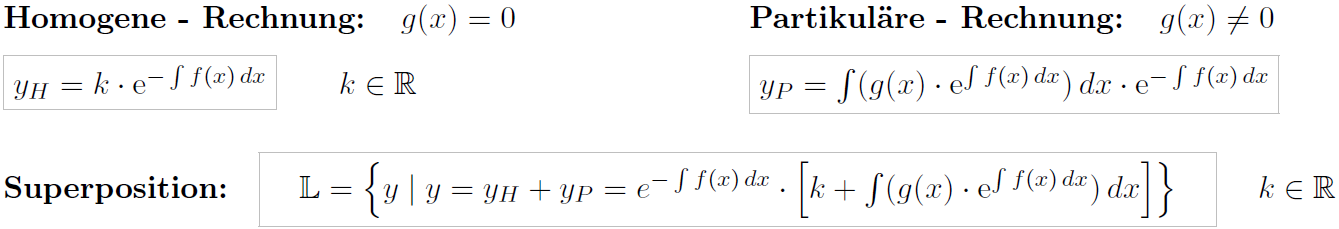
\includegraphics[width = 1.18\textwidth]{bilder/alg_DGL1.png}
	\end{minipage}
	\\
	\hline

\end{tabularx}	
\end{center}
\end{table}	
	% % % % % % % % % % % % % % % % % %
%DGL 2. Ordnung
% % % % % % % % % % % % % % % % % %	
% % % % % % % % % % % % % % % % % %
% neue Seite

\begin{table}[h!]
\begin{center}

\begin{tabularx}{\textwidth}{|p{120pt}|X|}
\hline
\rowcolor{Gray}
\multicolumn{2}{|c|}{\textbf{DGL 2. Ordnung}\qquad \fb{S.564}}\\
\hline
	Form  & Lösung\\
\hline
	$y''+a_1\cdot y'+a_0\cdot y=g(x)$&
	Wie bei 1. Ordnung: $Y=y_H+y_p$ \newline
	Homogene DGL: $g(x)=0$ \qquad Inhomogene DGL: $g(x)\neq 0$\\
\hline
\hline
	\rowcolor{LightCyan}
	\multicolumn{2}{|c|}{Homogene DGL $\qquad y''+a_1\cdot y'+a_0\cdot y=0$}\\
	\multicolumn{2}{|c|}{Charakt. Polynom:
	$\qquad \lambda^2+a_1\cdot\lambda+a_0=0 \qquad$ von
	$\qquad y''+a_1\cdot y'+a_0\cdot y=0$ 
	$\qquad(\lambda_{1,2} = -\frac{a_1}{2} \pm \frac{\sqrt{a_1^2 - 4a_0}}{2})$}
	\\
	\hline
	
	\multicolumn{2}{|l|}{
	$
	D = \left(\frac{a_{1}}{2}\right)^{2}-a_{0} =
	\left\{
	\begin{aligned}
		D>0: & \qquad \lambda_{1,2}=-\frac{a_{1}}{2} \pm \sqrt{\left(\frac{a_{1}}{2}\right)^{2}-a_{0}} & \qquad \in \mathbb{R} & \qquad \text{ starke D"ampfung }
		\\
		D=0: & \qquad \lambda \quad=\quad-\frac{a_{1}}{2} & \qquad \in \mathbb{R} & \qquad \text{ aperiodischer Grenzfall }
		\\
		D<0: & \qquad \lambda_{1,2}=-\frac{a_{1}}{2} \pm j \sqrt{a_{0}-\left(\frac{a_{1}}{2}\right)^{2}} & \qquad \in \mathbb{C}  \backslash \mathbb{R} & \qquad  \text{ schwache Dämpfung / Schwingfall }
	\end{aligned} \right.
	$
	}
	\\
	\hline

	\multicolumn{2}{|l|}{$(D > 0)\qquad$Falls: $\lambda_1\neq \lambda_2$ und $\lambda_{1,2} \in R\qquad$: 
	$Y_H=Ae^{\lambda_1x}+Be^{\lambda_2x\qquad}$  
	$\rbrace$ starke Dämpfung}\\
	\hline
	
	\multicolumn{2}{|l|}{$(D = 0)\qquad$
	Falls: $\lambda_1=\lambda_2$ und $\lambda_{1,2} \in R\qquad$: 
	$Y_H=e^{\lambda_1x}(A+B\cdot x)\qquad$ 
	$\rbrace$ aperiodischer Grenzfall}\\
	\hline
	
	\multicolumn{2}{|l|}{$(D < 0)\qquad$ 
	Falls $y_{H}=A \cdot \mathrm{e}^{\lambda x}=A \cdot \mathrm{e}^{-\frac{a_{1}}{2} x} \cdot \mathrm{e}^{ \pm j \sqrt{|D|} x}=A \cdot \mathrm{e}^{-\frac{a_{1}}{2} x} \cdot[\cos (\sqrt{|D|} x) \pm j \sin (\sqrt{|D|} x)]$ 
	$\rbrace$ schwache Dämpfung / Schwingfall} \\
	
	(Eigen-)Frequenz&
	$\omega=\alpha=\dfrac{\sqrt{|a_1^2 - 4a_0|}}{2} \qquad \qquad \qquad \omega=\sqrt{|D|}=\sqrt{\left|\delta^{2}-a_{0}\right|}$\\
	
	Dämpungskonstante&
	$\delta=-\frac{a_{1}}{2}$\\
	
	Resonanz&
	$\delta$ und $\omega$ stimmen überein mit Störglied\\
\hline

\hline
	\rowcolor{LightCyan}
	\multicolumn{2}{|c|}{inhomogene DGL $\qquad y''+a_1\cdot y'+a_0\cdot y=g(x)$ }\\
	Grundlöseverfahren
	\newline\newline
	(Faltungsintegral)
	&
	\begin{compactenum}
		\item Homogene DGL lösen: $g(x)=0$ setzen $\rightarrow$ ergibt $Y_H$
		\item Anfangsbedingungen in Hom. DGL einsetzen. Wenn möglich: $x_0=0\quad \newline 
				y_H(x_0)=0 \newline  y_H'(x_0)=1 \qquad$
		\item A, B bestimmen
		\item  Einsetzen der Hom. Glg. in Faltungsintegral 
		$\Rightarrow\quad y_P(x)=\int\limits_{x_o}^{x} y_H(x+x_0-t)\cdot g(t)dt$
		\item $Y=y_H+y_P$
	\end{compactenum}\\

\hline
\end{tabularx}
% % % % % % % % % % % % % % % % % %
%Ansatz in Form des Störgliedes
% % % % % % % % % % % % % % % % % %
\begin{tabularx}{\textwidth}{|p{120pt}|X|}
	\hline
	Ansatz in Form des \newline
	Störgliedes
	&
	\begin{compactenum}
		\item Homogene DGL lösen: $g(x)=0$ setzen $\rightarrow$ ergibt $Y_H$
		\item g(x) in Störgliedtabelle suchen
		\item Fall bestimmen
		\item $y_P$ aus Tabelle ablesen
		\item $Y=y_H+y_P$
	\end{compactenum}\\
\end{tabularx}

\renewcommand{\arraystretch}{1.1}
\begin{tabularx}{\textwidth}{|p{270pt}|X|}
	\hline 	$\mathbf{g(x)=p_n(x)}$ & 
		($p_n(x)$ und $q_n(x)$ sind Polynome vom gleichen Grad)\\

	 \hline	Fall 1: $a_0\neq 0$:          & $y_P = q_n(x)$\\
		Fall 2: $a_0 = 0 , a_1\neq 0$:& $y_P=x\cdot q_n(x)$\\
		Fall 3: $a_0=a_1=0$:          & $y_P=x^2\cdot q_n(x)$\\
		($a_0$ und $a_1$ beziehen sich auf die \textbf{linke Seite} der DGL) & \\
	\hline
	\hline
 		$\mathbf{g(x)=e^{bx}\cdot p_n(x)}$ & \\
	\hline	Fall 1: $b$ nicht Nullstelle des char. Polynoms:    &
		$y_P=e^{bx}\cdot q_n(x)$\\
		Fall 2: $b$ einfache Nullstelle des char. Polynoms: &
		$y_P=e^{bx}\cdot x \cdot q_n(x)$\\
		Fall 3: $b$ zweifache Nullstelle des char. Polynoms:&
		$y_P=e^{bx}\cdot x^2\cdot q_n(x)$\\
	\hline
	\hline
		$\mathbf{g(x) = e^{\alpha x}(p_n(x)\cos \beta x + q_n(x)\sin \beta x)}$ & \\
	 \hline	Fall 1: $\alpha + j\cdot\beta$ \textbf{nicht Lösung} der charakteristischen Gleichung: &
		$y_p = e^{\alpha x}\cdot(r_n(x)\cdot\cos(\beta \cdot x) + s_n(x)\cdot\sin( \beta\cdot x))$ \\
		Fall 2: $\alpha + j\cdot\beta$ \textbf{Lösung} der charakteristischen Gleichung: &
		$y_p = e^{\alpha x}\cdot \textbf{x} \cdot(r_n(x) \cdot \cos(\beta\cdot x) + s_n(x) \cdot\sin(\beta\cdot x))$\\
	\hline
\end{tabularx}
\renewcommand{\arraystretch}{2}
\end{center}
\end{table}	


\begin{table}[h!]
\begin{center}

% % % % % % % % % % % % % % % % % %
%Vorgehen bei einer DGL in From des Störgliedes
% % % % % % % % % % % % % % % % % %	
\begin{tabularx}{\textwidth}{|p{25pt}|X|}
\hline
\multicolumn{2}{|c|}{\textbf{Vorgehen bei einer DGL in Form des Störgliedes}}\\
\hline
 	1. &$Y_H$ mit $\lambda_1$ und $\lambda_2$ berechnen\\
	2. & Ordnung $n$ anhand der r.h.s der DGL bestimmen
			Koeffizient $b$ anhand der r.h.s der DGL bestimmen\newline
			(Achtung kann aus mehreren Elementen bestehen z.B. $x^2e^x + x$; Superposition)\\
		
	3. &	Anhand der Störglied Tabellen $y_p$ bestimmen\\
	4. & 	$q_n = ax^n + bx^{n-1} + \dots + cx + d$\\
	5. & 	$y_p$ ableiten und in die \textbf{ l.h.s} der DGL einsetzen. $\qquad y_p'' + a_1 y_p' + a_0y_p = f(x)$\\
	6. & 	Koeffizienten bestimmen: $\textcolor{red}{x^2e^x}\cdot 18a + xe^x(6a + 12b) + e^x(2b + 6c) = \textcolor{red}{x^2e^x}$\newline
			\begin{tabular}{ll}
				$18a = 1$ & $18a$ kommt 1mal in der r.h.s vor\\
				$(6a + 12b) = 0$ & $(6a + 12b)$ kommt 0mal vor auf der r.h.s\\
				$(2b + 6c) = 0$ & $(2b + 6c)$ kommt 0mal vor auf der r.h.s
			\end{tabular}\\
	7. & 	Koeffizienten in $y_p$ einsetzen\\
	8. & 	Wenn das Störglied $f(x)$ aus mehreren Teilen besteht (z.B. $x^2e^x + x$), Störglied auseinander nehmen und in zwei Teile $x^2e^x$ und $x$ unterteilen und Schritt 3 - 6 wiederholen\\
	9. & 	$y = Y_H + y_{p1} + y_{p2} + \dots$\\

\hline
\end{tabularx}
\begin{tabularx}{\textwidth}{|p{120pt}|X|}
Superpositionsprinzip & $f(x)=c_1f_1(x)+c_2f_2(x)$\newline
$y_1$ ist spezielle Lösung der DGL $\qquad$
$y_1''+a_1\cdot y_1'+a_0\cdot y_1=c_1f_1(x)$ \newline
$y_2$ ist spezielle Lösung der DGL $\qquad$
$y_2''+a_1\cdot y_2'+a_0\cdot y_2=c_2f_2(x)$ \newline
dann ist $y_P=c_1y_1+c_2y_2$\\
\hline
\end{tabularx}

	% % % % % % % % % % % % % % % % % %
%DGL 1. Ordnung - Orthogonaltrajektorien
% % % % % % % % % % % % % % % % % %	
\begin{tabularx}{\textwidth}{|p{100pt}|X|}
	\hline
	\rowcolor{Gray}
	\multicolumn{2}{|c|}{\textbf{DGL 1. Ordnung}}\\
	\hline
		Orthagonaltrajektorien \newline
		
		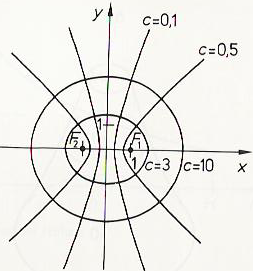
\includegraphics[width = 90pt]{bilder/orthoTrajekt_klein.png}	
		
		&
		Orthogonaltrajektorien sind die Normalen der DGL. Sie stehen senkrecht auf den Kurven die durch die DGL entstehen. \newline
		Die orthogonalen Trajektorien schneiden alle Kurven der gegebenen Kurvenschar
		$y=f(x,c)$ im rechten Winkel. \newline
					\textbf{Vorgehen:}
					\begin{compactenum}
						\item $y$ nach $c$ umstellen/ auflösen
						\item $y$ ableiten $\Rightarrow y'$
						\item in $y'$ Gleichung (entweder oder)
						$\begin{cases}
							c \text{ substitutieren/ ersetzen} \Rightarrow \text{DGL: F(x,y,y')}\\
							y \text{ Gleichung in } y' \text{ Gleichung einsetzen}
						\end{cases}$
						\item $y'$ durch $-\frac{1}{'y}$ ersetzen.
						\item DGL auflösen (sofern nötig...)
					\end{compactenum}
				\begin{minipage}{0.2\textwidth}
					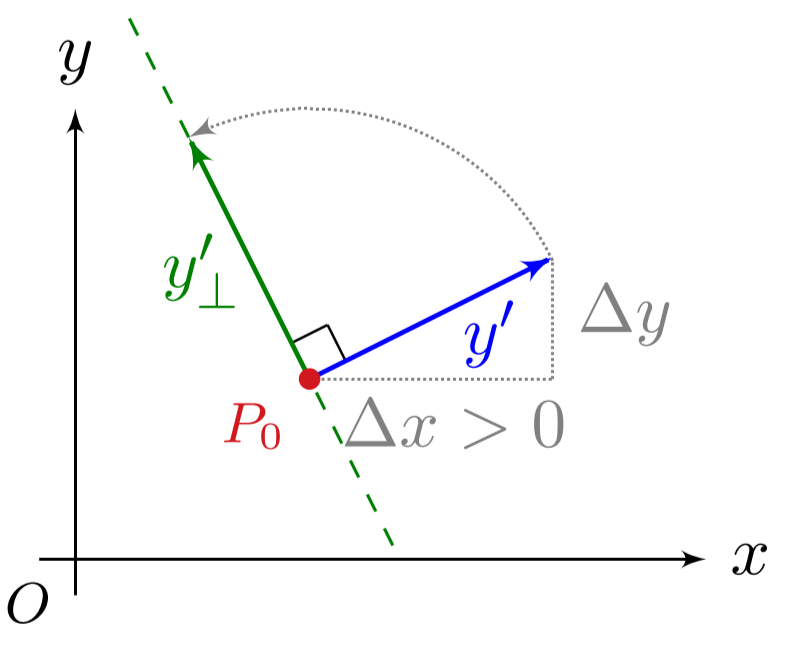
\includegraphics[width = \textwidth]{bilder/orthoTrajekt_Formel}
				\end{minipage} 
				\begin{minipage}{0.3\textwidth}
					\begin{tabular}{c|c}
						Kartesische Koordinaten: & Polarkoordinaten \\
						$y^{\prime}=f(x, y) \quad \Rightarrow \quad y_{\perp}^{\prime}=-\frac{1}{f(x, y)}$ &
						$r^{\prime}=f(r, \varphi) \quad \Rightarrow \quad r_{\perp}^{\prime}=-\frac{r^{2}}{f(r, \varphi)}$
					\end{tabular}
				\end{minipage}
				
				\\
	\hline
\end{tabularx}
		%		\end{minipage}%
%		\begin{minipage}{.8\textwidth}
%			Die orthogonalen Trajektorien schneiden alle Kurven der gegebenen Kurvenschar
%			$y=f(x,c)$ im rechten Winkel.\\

%		\end{minipage}



\end{center}
\end{table}	

	\begin{table}[h!]
\begin{center}

% % % % % % % % % % % % % % % % % %
%Lineare DGL n. Ordnung mit konstanten Koeffizienten
% % % % % % % % % % % % % % % % % %	
\begin{tabularx}{\textwidth}{|p{120pt}|X|}
	\hline
	\rowcolor{Gray}
	\multicolumn{2}{|c|}{\textbf{Lineare DGL n. Ordnung mit konstanten Koeffizienten}\qquad \fb{S.571}}\\
	\hline
	Form & $\sum\limits_{k=0}^na_ky^{(k)}= y^{(n)}+a_{n-1}\cdot y^{(n-1)}+\ldots +a_0\cdot y=g(x)$\\
	\hline
\end{tabularx}
\renewcommand{\arraystretch}{1}
\begin{tabularx}{\textwidth}{|p{130pt}p{240pt}X|}
	\multicolumn{3}{|c|}{n-verschiedene Homogene Lösungen}\\
	\hline
	\underline{Fall 1: r reelle Lösungen} & & Starke Dämpfung / Kriechfall\\
	$\lambda_{r-1} \neq \lambda_r $ & $y_1=A_1\cdot e^{\lambda_1x}$, $y_2=A_2\cdot e^{\lambda_2x}$, \ldots ,$y_r= A_r\cdot e^{\lambda_rx}$ & \\
	\\
	$\lambda_{r-1} = \lambda_r \qquad (\Rightarrow \lambda)$
	& $y_1=A_1\cdot e^{\lambda_x}$, $y_2=A_2\cdot x\cdot e^{\lambda x}$, \ldots,$y_r=A_r\cdot x^{r-1}\cdot e^{\lambda x}$ & \\ 
	\\
	\\
	\underline{Fall 2: $k$ komplexe Lösungen} & & Schwache Dämpfung / \\
	$ \lambda_{1,2}=\alpha \pm j\beta \neq \lambda_{k,k-1}$ & $y_k=e^{\alpha x}[A_k\cdot\cos(\beta\cdot x) + B_k\cdot\sin(\beta\cdot x)]$ & Schwingfall\\
	\\
	$ \lambda_{1,2}=\alpha \pm j\beta = \lambda_{k,k-1}$ & $y_1=e^{\alpha x}[A_1\cdot\cos(\beta\cdot x) + B_1\cdot\sin(\beta\cdot x)]$	&  \\
	 & $y_2=x \cdot e^{\alpha x}[A_2\cdot\cos(\beta\cdot x) + B_2\cdot\sin(\beta\cdot x)]$ & \\
	 & $ \ldots = \ldots $ & \\
	 & $y_k=x^k \cdot e^{\alpha x}[A_k\cdot\cos(\beta\cdot x) + B_k\cdot\sin(\beta\cdot x)]$ & (k-fache Resonanz) \\
	\\
	\multicolumn{3}{|l|}{$Y_H = y_1+ y_2+ y_3+... + y_n$}\\
	\hline
\end{tabularx}
\renewcommand{\arraystretch}{2}

% % % % % % % % % % % % % % % % % %
%Allgemeinste Lösung des partikulären Teils
% % % % % % % % % % % % % % % % % %	
\begin{tabularx}{\textwidth}{|p{300pt}|X|}
\hline
	\multicolumn{2}{|c|}{Allgemeinste Lösung des partikulären Teils}\\
\hline
	\multicolumn{2}{|c|}{$\underbrace{\sum_{k=0}^n a_k y^{(k)}}_{f(y,y',y'',\ldots)} = \underbrace{e^{\alpha x} (p_{m1}(x) \cos (\beta x) + q_{m2}(x) \sin (\beta x))}_{\text{Störglied}} \qquad \lambda \text{ aus Homogenlösung}$}\\
\hline
	Unterscheide die Lösungen des charakteristischen Polynoms ($\lambda$): &
	mit m = max(m1, m2)\\

	Fall a: $\alpha + j\beta \neq \lambda$, so ist &
	$y_P = e^{\alpha x}(r_m(x)\cos(\beta x) + s_m(x) \sin(\beta x))$\\
	Fall b: $\alpha + j\beta$  ist u-fache Lösung von $\lambda$, so ist &
	$y_P = e^{\alpha x} x^u (r_m(x) \cos(\beta x) + s_m(x) \sin(\beta x))$\newline
	u-fache Resonanz\\
\hline
\end{tabularx}
% % % % % % % % % % % % % % % % % %
%Grundlöseverfahren
% % % % % % % % % % % % % % % % % %	
\begin{tabularx}{\textwidth}{|p{350pt}|X|}
\hline
	\multicolumn{2}{|c|}{Grundlöseverfahren}\\
\hline
	$\begin{pmatrix}
	g(x_0)=  & 0 & = & Ay_1(x_0)+By_2(x_0)+\ldots +Ny_n(x_0)\\
	g'(x_0)= & 0 & = & Ay_1'(x_0)+By_2'(x_0)+\ldots +Ny_n'(x_0)\\
	\vdots  & \vdots & \\                            
	g^{(n-1)}(x_0)= & 1 & = & Ay_1^{(n-1)}(x_0)+By_2^{(n-1)}(x_0)+\ldots
	+Ny_n^{(n-1)}(x_0)
	\end{pmatrix}$ &
	
	ergibt $c_1,\ldots ,c_n$ für\newline
	$y_{P}(x)=\int\limits_{x_0}^x{g(x+x_0-t)f(t)dt}$\\
\hline
\end{tabularx}

\begin{tabularx}{\textwidth}{|p{120pt}|X|}
	Anfangswertproblem&
	$y(x_0) = y_0 \qquad y'(x_0) = y_1 \qquad y''(x_0) = y_2 \qquad \dots \qquad y^{(n-1)}(x_0) = y_{n-1}$\\
\hline
\end{tabularx}
% % % % % % % % % % % % % % % % % %
%Lineare Differentialgleichungssysteme erster Ordnung mit konstanten Koeffizienten
% % % % % % % % % % % % % % % % % %	

\begin{tabularx}{\textwidth}{|p{8cm}X|}
\hline
\rowcolor{Gray}
\multicolumn{2}{|c|}{\textbf{Lineare Differentialgleichungssysteme erster Ordnung mit konstanten Koeffizienten}}\\
\hline
	\textbf{Form:}& $	\begin{matrix} \dot{x}=ax+by+f(t) \\ \dot{y}=cx+dy+g(t) \end{matrix} = \left(\begin{matrix} \dot{x} \\ \dot{y} \end{matrix}\right) = 
				\underbrace{\left(\begin{matrix} a & b \\ c & d \end{matrix}\right)}_{\text{M}} \left(\begin{matrix} x \\ y \end{matrix}\right) + \underbrace{\left(\begin{matrix} f(t) \\ g(t) \end{matrix}\right)}_{\text{Störvektor}}$ \\


	\textbf{Die allgem. Lösung ergibt sich aus der DGL:}&
	$\underbrace{\ddot{x}-(a+d) \cdot \dot{x}+\overbrace{(a\cdot d-b\cdot c)}^{\text{det(M)}}\cdot x=\dot{f}(t)-d\cdot f(t)+b \cdot g(t)}_{\text{normale DGL 2.Ordnung} \rightarrow \text{nach $x$ auflösen}}$\\
	& $y=\frac{1}{b}(\dot{x}-ax-f(t)))$\\

\textbf{Anfangsbedinungen:} &
$x_0(t_0) = x_0$ \\
& $\dot{x}_0(t_0) = a \cdot x_0(t_0) + b \cdot y_0(t_0) + f(t_0) = a \cdot x_0 + b \cdot y_0 + f(t_0) $\\
\hline
\multicolumn{2}{|c|}{\textbf{Anordnung beachten!} Gesuchte Grösse immer zu oberst (in diesem Fall ist die gesuchte Grösse $x$)}\\
\hline
\end{tabularx} 



\end{center}
\end{table}	
\end{document}
